\subsection{System Characteristics}
\label{sec:SystemCharacteristics}

\subsubsection{Steady State}
\label{sub:SteadyState}

The steady state response of the system was determined by setting the duty cycle of the LED to all values in the PWM range 0--255. \textcolor{red}{Each sample was acquired \SI{200}{\milli\second} after the previous one so that the system had time to reach a steady state. This is an adequate time between samples because $RC$ constant of the detector circuit in \autoref{fig:setup_LDR_circuit} is $\tau = R_2C_1 = \SI{60}{\milli\second}$ and \SI{400}{\milli\second} amounts to more than $3\tau$. The reason why $R_2$ is in the time constant and not $R_3$ is because the PWM value was incremented and hence $C_1$ charges via $R_2$. If the data was acquired while decrementing the PWM value $R_3$ would be used instead.}

% explain R_2's value above?

A graph of the acquired data can be seen in \autoref{fig:steady_state}. We conclude that the resistance of the LDR does not vary linearly with the duty cycle on the LED. Nonetheless it is possible to obtain a linear function relating the input an output of the system, as described in \ref{subsubsec:LDR_model}.

\begin{figure}[h]
    \centering
    \resizebox{\textwidth}{!}{% Title: glps_renderer figure
% Creator: GL2PS 1.3.8, (C) 1999-2012 C. Geuzaine
% For: Octave
% CreationDate: Tue Dec 29 23:09:54 2015
\setlength{\unitlength}{1pt}
\begin{picture}(0,0)
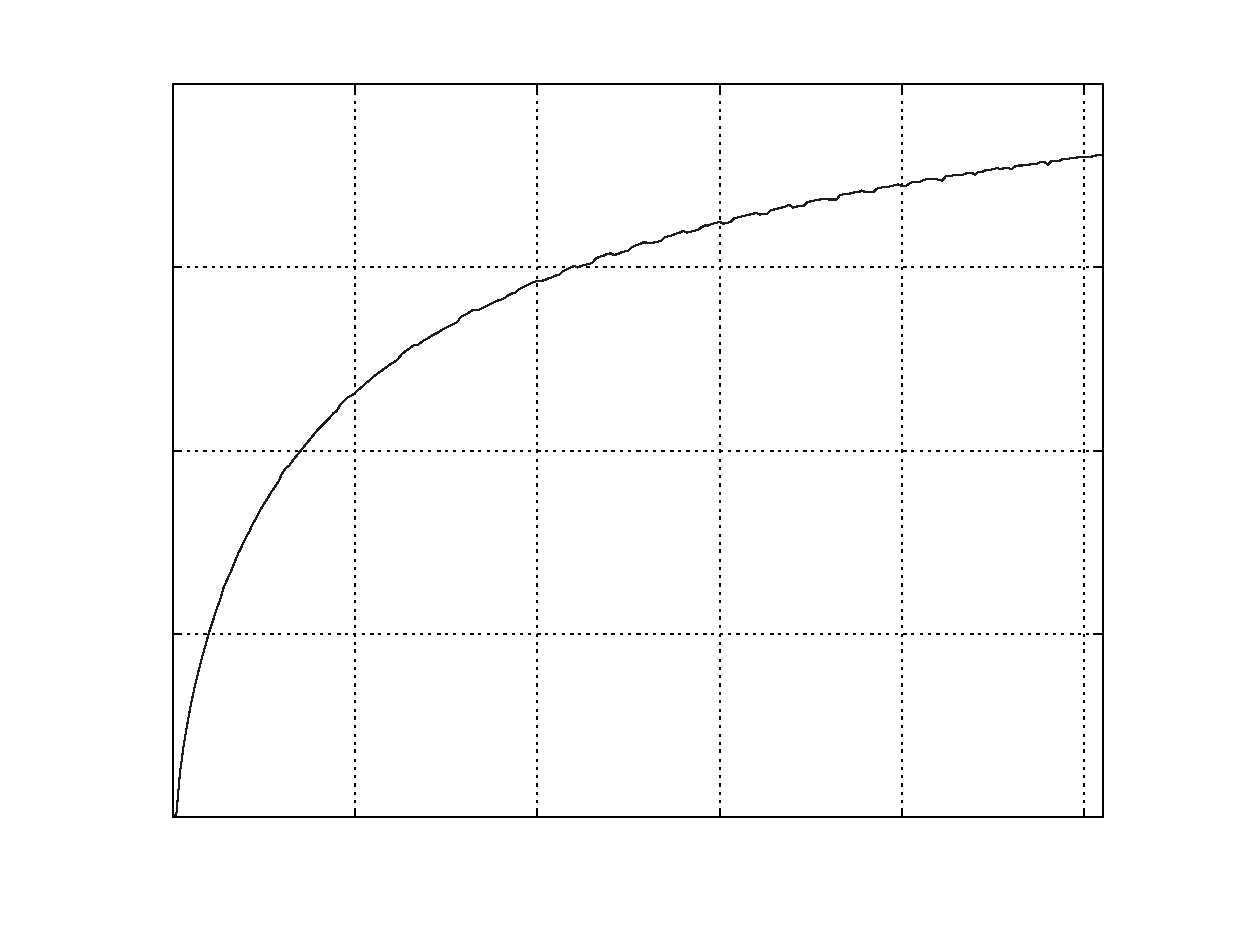
\includegraphics{img/steady_state-inc}
\end{picture}%
\begin{picture}(576,432)(0,0)
\fontsize{10}{0}
\selectfont\put(74.88,42.5189){\makebox(0,0)[t]{\textcolor[rgb]{0,0,0}{{0}}}}
\fontsize{10}{0}
\selectfont\put(162.409,42.5189){\makebox(0,0)[t]{\textcolor[rgb]{0,0,0}{{50}}}}
\fontsize{10}{0}
\selectfont\put(249.939,42.5189){\makebox(0,0)[t]{\textcolor[rgb]{0,0,0}{{100}}}}
\fontsize{10}{0}
\selectfont\put(337.468,42.5189){\makebox(0,0)[t]{\textcolor[rgb]{0,0,0}{{150}}}}
\fontsize{10}{0}
\selectfont\put(424.998,42.5189){\makebox(0,0)[t]{\textcolor[rgb]{0,0,0}{{200}}}}
\fontsize{10}{0}
\selectfont\put(512.527,42.5189){\makebox(0,0)[t]{\textcolor[rgb]{0,0,0}{{250}}}}
\fontsize{10}{0}
\selectfont\put(69.8755,47.52){\makebox(0,0)[r]{\textcolor[rgb]{0,0,0}{{0}}}}
\fontsize{10}{0}
\selectfont\put(69.8755,135.54){\makebox(0,0)[r]{\textcolor[rgb]{0,0,0}{{1}}}}
\fontsize{10}{0}
\selectfont\put(69.8755,223.56){\makebox(0,0)[r]{\textcolor[rgb]{0,0,0}{{2}}}}
\fontsize{10}{0}
\selectfont\put(69.8755,311.58){\makebox(0,0)[r]{\textcolor[rgb]{0,0,0}{{3}}}}
\fontsize{10}{0}
\selectfont\put(69.8755,399.6){\makebox(0,0)[r]{\textcolor[rgb]{0,0,0}{{4}}}}
\fontsize{10}{0}
\selectfont\put(298.08,31.5188){\makebox(0,0)[t]{\textcolor[rgb]{0,0,0}{{PWM value (0--255)}}}}
\fontsize{10}{0}
\selectfont\put(59.8755,223.56){\rotatebox{90}{\makebox(0,0)[b]{\textcolor[rgb]{0,0,0}{{Voltage at \texttt{A0} (\si{\volt})}}}}}
\end{picture}
}
    \caption{Steady state voltage at pin \texttt{A0} as a function of the duty cycle of the LED}
    \label{fig:steady_state}
\end{figure}

\subsubsection{Modeling the LDR}
\label{subsubsec:LDR_model}

Since the steady state plot in \autoref{fig:steady_state} reveals that the system is nonlinear it is useful to understand why. The main sources from nonlinearity should result from the LED, the LDR or a combination of both.

% TODO put full datasheet in an annex?

With that in mind the LDR datasheet was analysed. On it the graph in \autoref{fig:LDR_datasheet} can be found. This graph gives a range of values for the resistance of the LDR for each value of incident illuminance. To produce an equation that models the LDR resistance as a function of illuminance the resistance value used for the model is the mean of the maximum and minimum values given for each illuminance. The final result should be a function which produces a line that crosses the middle of the dark region in \autoref{fig:LDR_datasheet}. Note the axis of the figure are both in logarithmic scale. The considered points to obtain this linear function (in a log-log reference) were $(L_1, R_1) = (\SI{100}{\lux}; \SI{2.5}{\kilo\ohm})$ and $(L_2, R_2) = (\SI{1}{\lux}; \SI{60}{\kilo\ohm})$. The model will be an equation in the form
\begin{equation} \label{eq:log-log_line}
    \log_{10} R_{LDR} = a \log_{10} L + b.
\end{equation}

\begin{figure}[h]
    \centering
    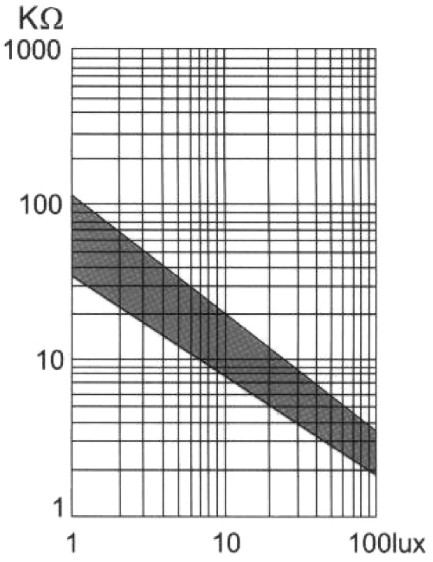
\includegraphics[width=.4\textwidth]{img/LDR_datasheet}
    \caption{LDR resistance as a function of illuminance \\ according to the GL5528's datasheet}
    \label{fig:LDR_datasheet}
\end{figure}

We can substitute $(L_1, R_1)$ and $(L_2, R_2)$ in \eqref{eq:log-log_line} to obtain the system of equations
\begin{equation} \label{eq:log-log_line_system}
    \begin{bmatrix}
	\log_{10}R_1 \\ \log_{10}R_2
    \end{bmatrix}
    =
    \begin{bmatrix}
	\log_{10}L_1  &  1 \\
	\log_{10}L_2  &  1
    \end{bmatrix}
    \begin{bmatrix}
	a \\ b
    \end{bmatrix}.
\end{equation}
By solving the system the values $a \approx -0.6901$ and $b \approx 4.7782$ are obtained for this case.

With the values for $a$ and $b$ and \eqref{eq:log-log_line} it is possible to plot the graph in \autoref{fig:LDR_model} which models the LDR characteristic, as desired. Using \eqref{eq:log-log_line} it is possible to obtain the incident illuminance ($L$) from the resistance of the LDR $R_{LDR}$
\begin{equation} \label{eq:Rldr_to_lux}
    L = 10^{-\frac{b}{a}} R_{LDR}^{\frac{1}{a}} .
\end{equation}
And since in a steady state
\begin{equation} \label{eq:VA0_to_Rldr}
    R_{LDR} = \frac{V_S R_3}{V_{\texttt{A0}}} - R_3 ,
\end{equation}
we can substitute \eqref{eq:VA0_to_Rldr} in \eqref{eq:Rldr_to_lux} and apply the new equation to the plot in \autoref{fig:steady_state} to produce the plot in \autoref{fig:pwm_to_lux} which relates the duty cycle of the LED to the illuminance measured by the LDR. We can conclude that the illuminance varies linearly with the duty cycle applied to the LED.

\begin{figure}[h]
    \centering
    \resizebox{\textwidth}{!}{% Title: glps_renderer figure
% Creator: GL2PS 1.3.8, (C) 1999-2012 C. Geuzaine
% For: Octave
% CreationDate: Tue Dec 29 00:54:08 2015
\setlength{\unitlength}{1pt}
\begin{picture}(0,0)
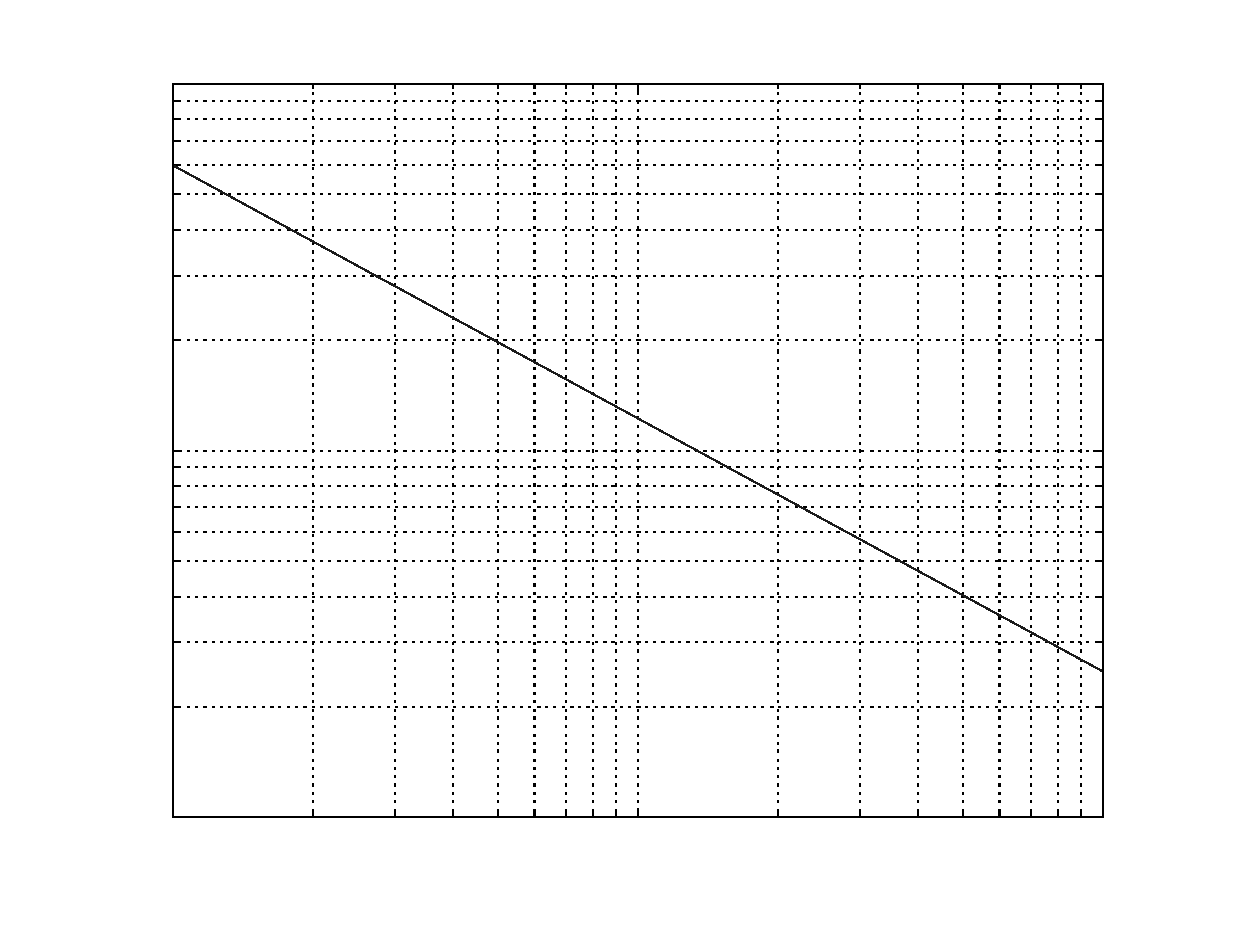
\includegraphics{img/LDR_model-inc}
\end{picture}%
\begin{picture}(576,432)(0,0)
\fontsize{10}{0}
\selectfont\put(74.88,42.5189){\makebox(0,0)[t]{\textcolor[rgb]{0,0,0}{{1e+0}}}}
\fontsize{10}{0}
\selectfont\put(298.08,42.5189){\makebox(0,0)[t]{\textcolor[rgb]{0,0,0}{{1e+1}}}}
\fontsize{10}{0}
\selectfont\put(521.28,42.5189){\makebox(0,0)[t]{\textcolor[rgb]{0,0,0}{{1e+2}}}}
\fontsize{10}{0}
\selectfont\put(69.8755,47.52){\makebox(0,0)[r]{\textcolor[rgb]{0,0,0}{{1e+3}}}}
\fontsize{10}{0}
\selectfont\put(69.8755,223.56){\makebox(0,0)[r]{\textcolor[rgb]{0,0,0}{{1e+4}}}}
\fontsize{10}{0}
\selectfont\put(69.8755,399.6){\makebox(0,0)[r]{\textcolor[rgb]{0,0,0}{{1e+5}}}}
\fontsize{10}{0}
\selectfont\put(298.08,31.5188){\makebox(0,0)[t]{\textcolor[rgb]{0,0,0}{{Illuminance (\si{\lux})}}}}
\fontsize{10}{0}
\selectfont\put(39.8755,223.56){\rotatebox{90}{\makebox(0,0)[b]{\textcolor[rgb]{0,0,0}{{Resistance (\si{\ohm})}}}}}
\end{picture}
}
    \caption{Model for the resistance of the LDR as function of the incident illuminance}
    \label{fig:LDR_model}
\end{figure}

\begin{figure}[h]
    \centering
    \resizebox{\textwidth}{!}{% Title: glps_renderer figure
% Creator: GL2PS 1.3.8, (C) 1999-2012 C. Geuzaine
% For: Octave
% CreationDate: Mon Dec 28 19:17:53 2015
\setlength{\unitlength}{1pt}
\begin{picture}(0,0)
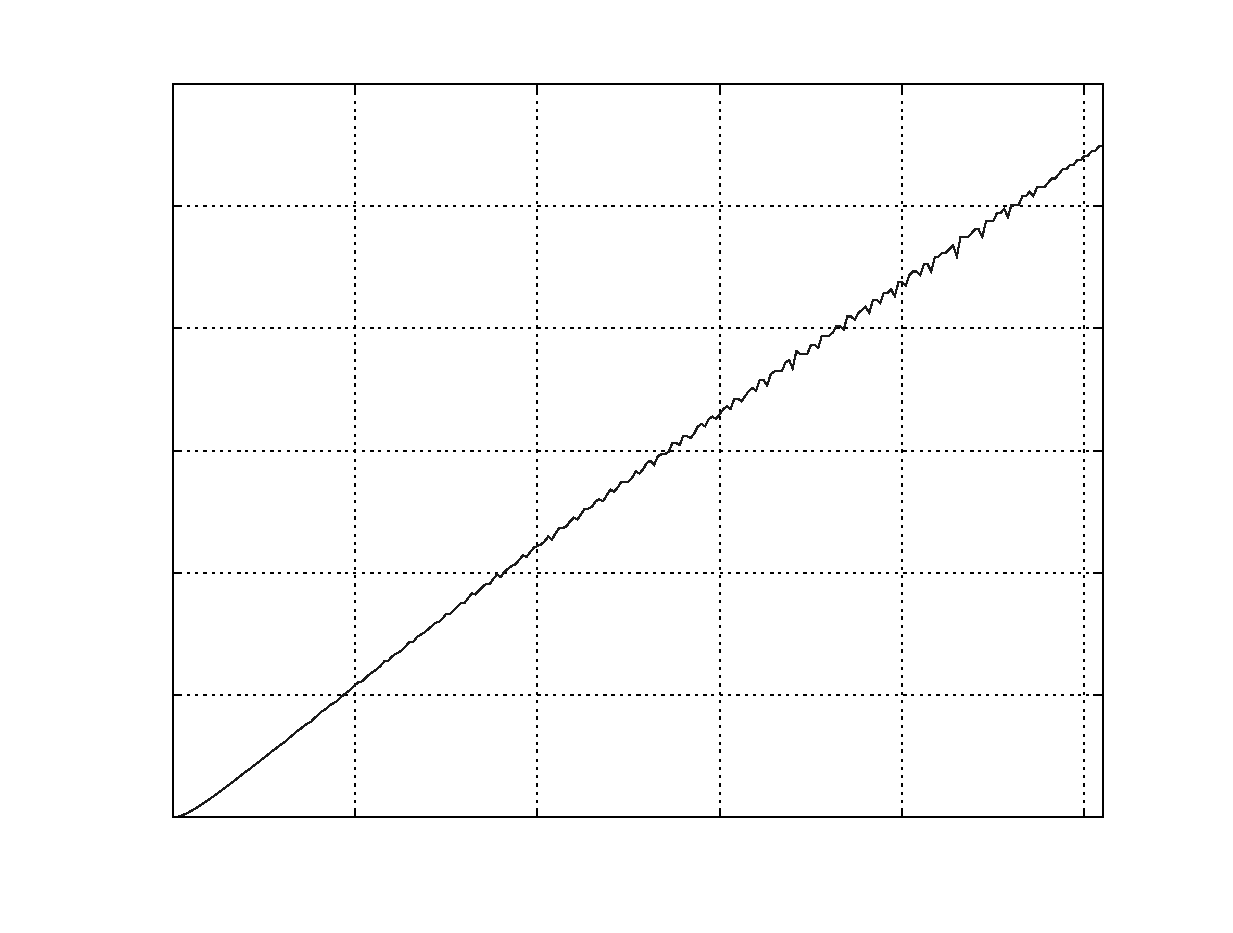
\includegraphics{img/pwm_to_lux-inc}
\end{picture}%
\begin{picture}(576,432)(0,0)
\fontsize{10}{0}
\selectfont\put(74.88,42.5189){\makebox(0,0)[t]{\textcolor[rgb]{0,0,0}{{0}}}}
\fontsize{10}{0}
\selectfont\put(162.409,42.5189){\makebox(0,0)[t]{\textcolor[rgb]{0,0,0}{{50}}}}
\fontsize{10}{0}
\selectfont\put(249.939,42.5189){\makebox(0,0)[t]{\textcolor[rgb]{0,0,0}{{100}}}}
\fontsize{10}{0}
\selectfont\put(337.468,42.5189){\makebox(0,0)[t]{\textcolor[rgb]{0,0,0}{{150}}}}
\fontsize{10}{0}
\selectfont\put(424.998,42.5189){\makebox(0,0)[t]{\textcolor[rgb]{0,0,0}{{200}}}}
\fontsize{10}{0}
\selectfont\put(512.527,42.5189){\makebox(0,0)[t]{\textcolor[rgb]{0,0,0}{{250}}}}
\fontsize{10}{0}
\selectfont\put(69.8755,47.52){\makebox(0,0)[r]{\textcolor[rgb]{0,0,0}{{0}}}}
\fontsize{10}{0}
\selectfont\put(69.8755,106.2){\makebox(0,0)[r]{\textcolor[rgb]{0,0,0}{{10}}}}
\fontsize{10}{0}
\selectfont\put(69.8755,164.88){\makebox(0,0)[r]{\textcolor[rgb]{0,0,0}{{20}}}}
\fontsize{10}{0}
\selectfont\put(69.8755,223.56){\makebox(0,0)[r]{\textcolor[rgb]{0,0,0}{{30}}}}
\fontsize{10}{0}
\selectfont\put(69.8755,282.24){\makebox(0,0)[r]{\textcolor[rgb]{0,0,0}{{40}}}}
\fontsize{10}{0}
\selectfont\put(69.8755,340.92){\makebox(0,0)[r]{\textcolor[rgb]{0,0,0}{{50}}}}
\fontsize{10}{0}
\selectfont\put(69.8755,399.6){\makebox(0,0)[r]{\textcolor[rgb]{0,0,0}{{60}}}}
\fontsize{10}{0}
\selectfont\put(298.08,31.5188){\makebox(0,0)[t]{\textcolor[rgb]{0,0,0}{{PWM value (0--255)}}}}
\end{picture}
}
    \caption{Illuminance detected by the LDR in function of the duty cycle of the LED}
    \label{fig:pwm_to_lux}
\end{figure}


\subsubsection{Step Response}
\label{sub:StepResponse}

To plot the step response of the system an Arduino program was written that to produce a step and acquire data to be ploted. In this script the LED is first turned off for \SI{1}{\second} so that the capacitor ``fully'' discharges. Then a step is applied to the system by setting the LED duty cycle to 0.5. A sample is acquired and sent to the computer approximately every \SI{1.35}{\milli\second}. The readings are converted to Volt and the result is \autoref{fig:step_response}.

An inflection point can be perceived early in the step response. From this follows that the system's order must be at least second degree. The detector in \autoref{fig:setup_LDR_circuit} includes a capacitor, which must introduce a pole. Therefore an experiment was made which consisted simply in removing the capacitor and acquiring the step response again. The result is shown in \autoref{fig:step_response_no_capacitor} where it can be seen that the aforementioned inflection does not exist. It is also noticable that introducing the capacitor does filter high frequency noise, as expected. Therefore introducing the capacitor improves the readings but makes the system order increase. Nonethess the capacitor value can be changed allowing to control the pole position and cutoff frequency.

Assuming that the system can be approximated to a first order system of the form $G(s) = K_0/(1+s\tau)$ the system can be modelled by finding the static gain $K_0$ and the time constant $\tau$. $K_0$ is calculated as the ratio of the output and the input under steady state; the time constant is the time the system takes to reach $1-e^{-1} \approx 63 \%$ of its final value. Therefore for \autoref{fig:step_response} the static gain is $3.08/2.5 = 1.232$ and the time constant is approximately $\SI{42}{\milli\second}.

\begin{figure}[h]
    \centering
    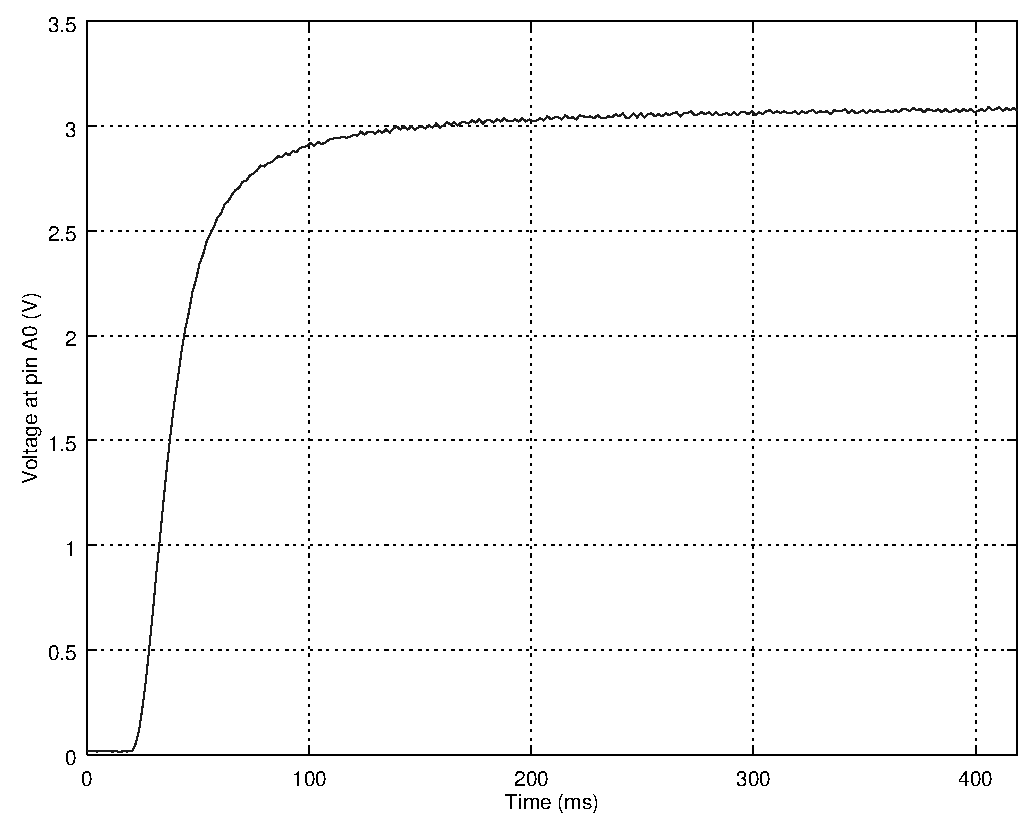
\includegraphics[width=.85\textwidth]{img/step_response}
    \caption{Response of the system to a step with 50\% duty cycle applied at time \SI{20}{\milli\second}}
    \label{fig:step_response}
\end{figure}

\begin{figure}[h]
    \centering
    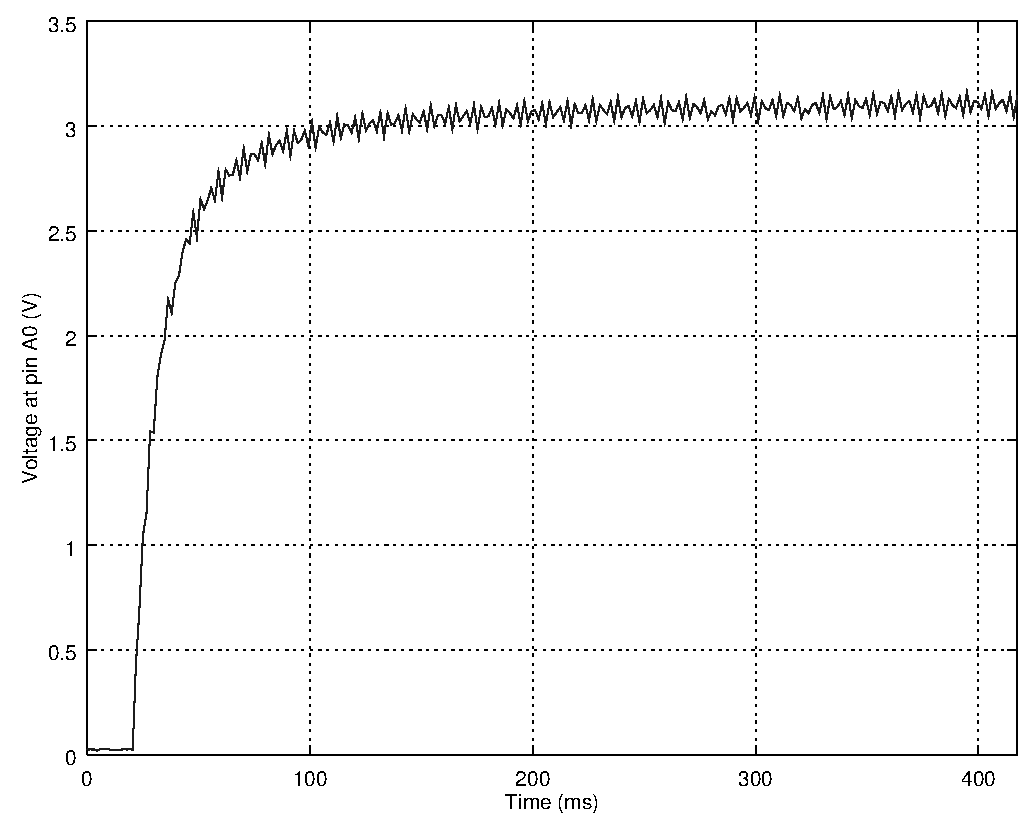
\includegraphics[width=.85\textwidth]{img/step_response_no_capacitor}
    \caption{}
    \label{fig:step_response_no_capacitor}
\end{figure}

\subsubsection{Incremental Response}
\label{sub:IncrementalResponse}

\begin{figure}[h]
    \centering
    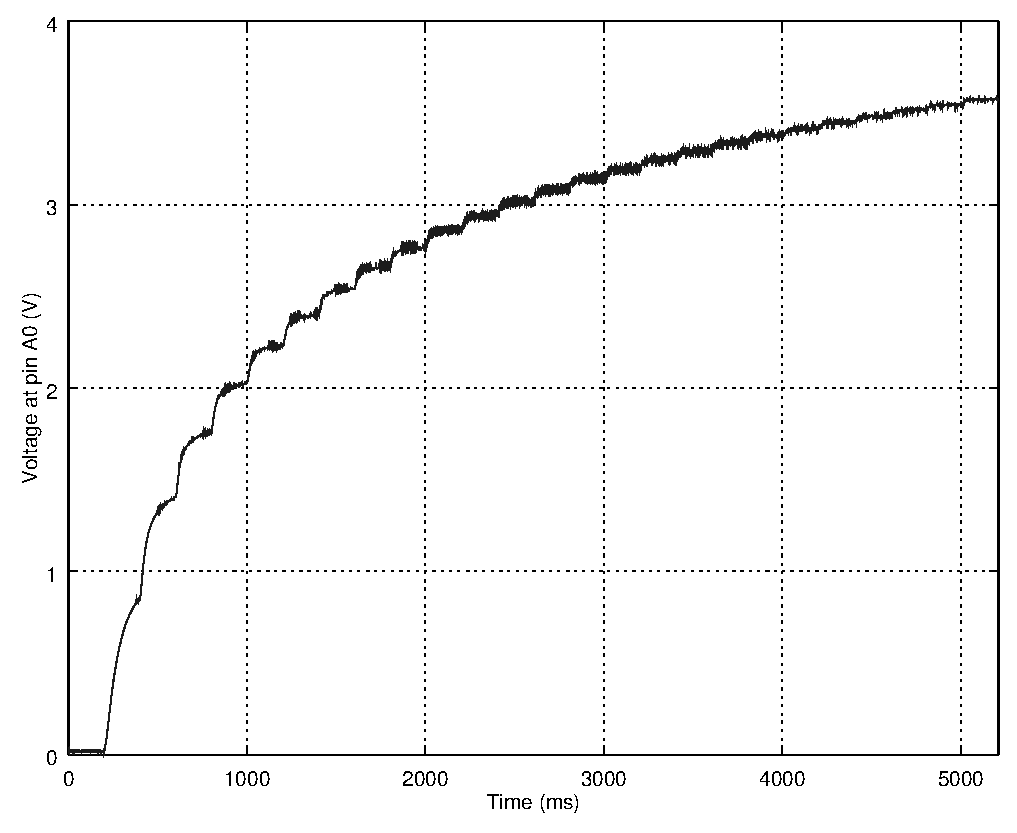
\includegraphics[width=.85\textwidth]{img/incstep_response}
    \caption{}
    \label{fig:incstep_response}
\end{figure}

